\chapter{Background}
\label{chap:background}
In this chapter the background and motivation for the study is introduced. This is followed by a section describing related work.

The work conducted in this thesis draws on knowledge from several fields of research. 

In contrast, the fields of Big Data, NoSQL, and polyglot persistence are newer. Knowledge from these fields are used to address the problem, define its solution and to assess feasibility. 

%------------------------------------------

\section{Related Work}

\subsection{Big Data}
%--Stycken i denna subsektion måste refaktoreras.
Since the emergence of the internet, big data is the phenomenon which has received the most attention by the computing industry \cite{bigDataWarehouse}. Today's popularity for big data is mainly derived from the current maturity in technologies combined with the ongoing decline in hardware costs \cite{bigDataWarehouse, bigDatabigAn}. This has led to the development of systems which enable the processing and handling of big data \cite{bigDataWarehouse}.

When traditional relational databases are used, analytics can only use small data sets to create models. With big data and its technologies, analytics now has the possibility to use far more data when creating predictive models. As described in \cite{bigDatabigAn}, using traditional relational databases lets you only see the tip of the iceberg, not what is under the surface. Big data gives analytics the ability of seeing the whole iceberg, even below the surface. With the capability to gather this massive amount of data, more intelligence can be mined from the data which can, if done right, be translated into business value \cite{bigDataMane}.

There are three characteristics that describes big data; volume, velocity and variety. Volume is the quantity of data. As an example, Walmart gathers more than 2.5 petabytes of customer transaction data per hour \cite{bigDataMane}. The velocity of data gathering should be nearly real-time, which enables the organization to be agile. Data is gathered from different sources or has different structures which gives more data points to correlate.

If any of these three characteristics are so extreme that they can't be processed using traditional technologies, it is considered to be big data \cite{bigDataWarehouse}. The boundary of when data becomes big data is influenced by which sector a system is in use. It is always in movement along with advancements in technology for that sector \cite{bigDatabigAn}. 

%In the case of CIMS, the volume can't be handled by the traditional database in use today.

%-------------------------------------------
\subsection{NoSQL databases}
Catell \cite{Catell} provides an overview of the current dialogue in the database world, primarily regarding big data trends and how to address the problem of scalability depending on technology and applications. The paper focuses on four different categories of databases; key value stores, document stores, extensible document stores and relational databases. Out of these, the first three fall under the category of NoSQL databases. Differences with traditional SQL databases typically boils down to trade-offs made about consistency in favour of scalability and flexible schemas. NoSQL databases have been designed primarily to meet modern demands on online applications that need to handle a large amount of concurrent users and storing of large amounts of possibly unstructured data \cite{Catell}.
As described above, a common way of comparing NoSQL and SQL databases is in terms of consistency and demands on it. SQL databases typically have ACID \cite{Mullins} transactions. ACID transactions are strict in the sense that they ensure that the every user always has exactly the same view of the database. Such constraints are very important for some use cases like the handling of banking transactions but less important for others, such as status updates in a social network.

When consistency can be relaxed, weaker constraints can be employed, given rise to the BASE \cite{Catell} acronym. Databases using this approach are eventually consistent, meaning updates will eventually propagate throughout the system. The idea is that when relaxing consistency, much greater performance and scalability is possible \cite{Catell}.

The NoSQL databases mentioned in \cite{Catell} provides scalability by horizontal scaling in a distributed manner, meaning that the data in the database can be spread on multiple servers. This distribution of data among multiple servers enables the database to meet the modern demands in both throughput and scalability \cite{Abadi} mentioned earlier. A distributed service is often designed with the desire to achieve three key characteristics; consistency, availability, and partition-tolerance \cite{Brewer}, but these are together impossible to achieve in a distributed environment \cite{Brewer}. Therefore a prioritisation must be made, a distributed database system can only posses two out of these three characteristics, in \cite{Brewer} called the CAP theorem. Due to the prioritisation made by the NoSQL variants mentioned in \cite{Catell}, they achieve scalability and availability in favour for consistency. 

The scope of \cite{Catell} covers SQL and NoSQL variants that address scalability by horizontal scaling. NoSQL databases are typically built with horizontal scaling in mind while for SQL variants, like MySQL, horizontal scaling has been added as a feature later in the life of the product.

Four different categories of NoSQL data stores mentioned in \cite{Catell} and \cite{NoSQLDistilled} are described in the sections below.

\hiddensubsubsection{Key value stores}

Key value stores uses a key-value index as structure, each value corresponds to a key which is used for lookups and deletes for that value\cite{Catell}. The data model used is a map or dictionary, which is simpler compared to a relational table and gives a faster query speed compared to a relational database \cite{NoSQLSurvey}. 

\hiddensubsubsection{Document stores}

Compared with the key value store where the key is used for lookups, a document store uses a query based on the structure of the document combined with certain attributes like Id in order to retrieve the data. The structure of the documents in a document store does not need to be defined in forehand and the structure of the documents does not need to be homogeneous, thereby the document store is said to be schemaless \cite{NoSQLDistilled}. The data structure of a document is a hierarchical tree which can contain lists, nested objects and maps \cite{Catell, NoSQLDistilled}. Due to the freedom in a document's structure and depending on which document store used, there exists different techniques to model relations between objects in a document store, different techniques offer different benefits in form of performance, size on disk etc. 

\hiddensubsubsection{Graph Databases}

Many NoSQL databases mentioned in \cite{Catell} consists of large blobs with low coupling, graph databases is the opposite, graph databases consists of small records with high and complex coupling. A graph is a data structure containing nodes that are connected with arcs\cite{NoSQLDistilled}. This highly interconnected structure gives the ability to query information based on the relations between nodes, for instance "find the parts included in product X that were manufactured by Y and shipped by Z". The relational databases would model these relations with foreign keys, but when querying complex relationships, the joins required becomes heavily performance demanding. The querying and traversal between the relationships becomes efficient and cheap in graph databases compared to the relational databases \cite{NoSQLDistilled}.

\hiddensubsubsection{Column-Family Stores}
Categorized as extensible document stores by \cite{Catell}. 

%---------------------------------------------

\subsection{Polyglot persistence}

There is a consensus in contemporary database literature that relational databases are not going to go away anytime soon \cite{Catell, NoSQLDistilled, NoSQLSurvey}. They are, however, no longer the one and only option for every problem. Instead, a contemporary viewpoint is that no data model can and should have the purpose of describing all kinds of domains \cite{NoSQLDistilled, NoSQLSurvey}. In practise this means that trying to model all data to fit into one kind of database, relational or otherwise, is not a prudent task. This problem is known in literature as impedance mismatch \cite{ORM}. Many strategies \cite{ORM} exist for overcoming it where a more recent one is the concept of polyglot persistence \cite{NoSQLDistilled}. 

The word polyglot means something that is made up of several languages. In the field of software this is often meant to mean a system that is built with several different programming languages. Similarly, polyglot persistence means that a system leverages several different databases. Rarely does all the data of a software system match nicely with one kind of data model. So instead of using the same data model for everything, databases with different data models and traits are used for specific kinds of data within a system. That is in essence, the idea behind polyglot persistence. To illustrate, figure~\ref{fig:polyglot} shows a design example of an e-commerce platform where different types of data exist along with database choices that are well suited to store this data.

%The argument for polyglot persistence is simple; Use the right tool for the right job. This means storing data in the form it naturally exists in its domain. One implication is that a system should potentially be made up of multiple databases, where each database is designed for specific kinds of data and to solve specific problems.

Polyglot persistence is closely related to the rise in popularity of NoSQL databases. These databases should not be considered general purpose \cite{Catell, polyglotms} but should instead be used for solving specific problems involving specific kinds of data. For the purposes of this study, polyglot persistence is an interesting approach that warrants further investigation. Since use cases for live and historical data are different and the fact that the amount of collected historical data will grow forever, we believe that using different databases for live and historical data might be beneficial. 

%A typical use case for NoSQL is storing massive scale and potentially unstructured data. This is an area where relational databases historically have a problem \cite{Catell}.

% TODO: Rewrite and add more stuff.

%Many modern systems already use specialized storage options for different tasks. A common example is a web application leveraging a key value store as a cache in front of a relational database. (källa)

%Using multiple types of data stores in the same system has been coined polyglot persistence \cite{NoSQLDistilled}. What categorizes these modern systems is that they are flexible, performant and scalable. This comes with a price in the form of increased complexity and as such puts higher demands on developers and maintainers. 
%
%For the purpose of this thesis, NoSQL is simply interpreted as "Not Relational" and includes technologies such as XML databases. Polyglot SQL/XML has been around for a while, but XML as a data interchange format is increasingly unpopular \cite{JSONData}. Not a single technology described by \cite{Catell} actually store data as XML. For a modern polyglot persistence solution with a focus on scalability and interoperability with web applications, XML seems to be impractical. 
%
%Schram and Anderson \cite{MySQLToNoSQL} describe a project with emerging scalability and performance requirements that evolved towards polyglot persistence using Cassandra in combination with MySQL. The authors describe both the software architecture challenges and the data modelling challenges that were present during development.

\begin{figure}[h!]
\centering
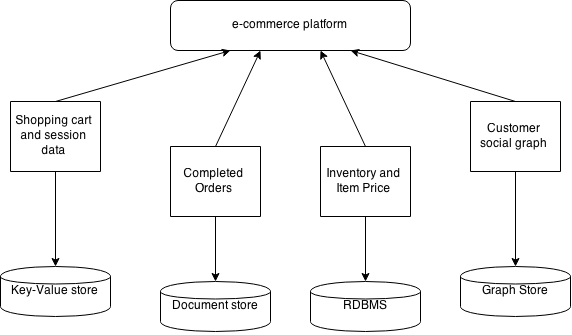
\includegraphics[scale=0.5]{figure/Polyglot.png}
\caption{Example implementation of polyglot persistence, seen in \cite{NoSQLDistilled}}
\label{fig:polyglot}
\end{figure}

%---------------------------------------------
%\subsection{Schema Evolution}
%%Vi skall försöka lyfta/hitta problem som Moon nämner och skriva de här. 
%Rham and Bernstein \cite{SchemaEvolutionBib} define schema evolution as the ability to change deployed schemas, where schemas are defined as metadata that formally describe artifacts such as databases. When schemas change, these changes may propagate to different parts of a system, such as it's source code or production data. As such, the main purpose of studying schema evolution is to find ways to minimize and automate propagation as much as possible \cite{SchemaEvolutionBib}.
%
%%Notable schema types are database schemas, XML schemas and ER/UML models. Schema evolution has been an active research topic for many years \cite{SchemaEvolutionBib} and is a 
%
%Curino et al. \cite{Moon09} discuss ways to handle data archiving in the context of evolving relational databases, describing two high level approaches. The first is to migrate historical data to new schema versions. The benefit is that both live and archived data can be retrieved using the same queries. The downside is that the archive is not a true historical representation since it imposes structural change on the historical data. The second approach is to keep the structure of all historical data. The archive is now a perfect historical representation but retrieval becomes harder and queries have to match old schemas \cite{Moon09}. A novel approach to the problem is finally described that is both structurally accurate and queried using the latest schema. This is achieved with a set of software components, one for example provides an XML-based data model for archiving data and another provides an interface for querying on this data.
%
%In \cite{Moon05}, schema evolution and querying of historical data is handled by saving the changes in each schema version, represented by the delta between different versions. Each delta is given a time stamp for their time of validity. The term V-Document is introduced and is used to describe a data format for storing the schema deltas in XML. Querying of V-Documents are done using XQuery. A mentioned drawback of this solution are the limitations in XQuery's performance and scalability \cite{Moon05}.
%
%Qiu et al.\ \cite{Co-evolutionOfSchemaAndCode} studies how frequent schema changes are, what schema changes typically consist of and the effects of schema changes on interacting systems. The study was done by conducting empirical analysis on open source software systems backed by a relational database. Results indicate that schema changes are frequent for these systems and that the most common changes consist of adding new columns or changing existing columns \cite{Co-evolutionOfSchemaAndCode}.
%
%A similar study to \cite{Co-evolutionOfSchemaAndCode} was conducted by Cleve et al.\ \cite{Oscar}. This case study focuses on an open source system within the health care sector. The goal was to investigate and understand the impact of schema evolution for one specific system which is significantly larger in terms of schema size than any system under study by \cite{Co-evolutionOfSchemaAndCode}. The main question the researchers ask is how can the history of a database schema be extracted, represented and exploited? It is argued that this knowledge can be used to help with migration of data to a non-relational data store used for research purposes as opposed to the OLTP workload the system under study was made for originally.
%
%Concepts from the approach used by \cite{Oscar} to build a historical schema representation are described. Based on developed tools, a four step approach to building the historical schema is given. In order for the approach to be viable, a versioning system needs to be in place for the system under study that keeps versions of the database schema over time. The four step approach then consists of extraction, parsing, comparison and finally visualisation.
%
%% Bättre övergång här
%There has also been work done on the topic of schema evolution outside of the realm of relational databases. Depending on the type of database, the coupling between database schemas and source code differs. When using a relational database, the database schema has to be changed before the code in the application is changed \cite{NoSQLDistilled}. In the case of a schemaless database, the code can evolve without evolving the database due to the schemaless databases capability of handling documents with different structure. It is important to note that the term schemaless does not mean that a schema does not exist but rather that data is self describing through an implicit schema. For schemaless databases, the only thing the application needs to handle is how to process documents with the old structure and documents with the new evolved structure \cite{NoSQLDistilled}. Depending on the structural impact of code change, documents in the database may need to be updated according to code evolution. 
%
%Schrezinger et al.\ \cite{EvolutionNoSQL} coins the term eager migration, where each entity is fetched from the database into the application then updated according to the new structure then written back to the database. This update of documents could get expensive if the database is handling a large amount of data. To avoid immediate resource consumption, incremental migration \cite{NoSQLDistilled}, also called lazy migration by \cite{EvolutionNoSQL} is suggested as a possible solution. With incremental migration, the application is capable of handling multiple versions of documents. Documents with an old structure is changed to the current structure at save time, thereby the migration of documents will be done over time. Some documents will never be migrated if they are not accessed by the application \cite{EvolutionNoSQL}. As \cite{EvolutionNoSQL} points out, the ability of an application to handle multiple document structures leads to increased code complexity and code debt.





